\documentclass{article}
\usepackage{graphicx}
\usepackage{color}
\color{black}

% Margin on left side of page is 1.0 inches plus \oddsidemargin.
\oddsidemargin  -0.65in
\evensidemargin  0pt
% Margin on top also appears to be 1.0 inches plus \topmargin (not checked).
\topmargin -0.7in
\headheight 0.0in
\headsep 0.0in
\marginparwidth 0pt
\marginparsep 0pt
\textwidth   7.5in
\textheight  10.5in

\title{CSE166 - Image Processing - Homework 7}
\author{Nitay Joffe}
\date{November 30, 2006}

\begin{document}
%\includegraphics[scale=1.0]{CSE166CoverSheet.pdf}
\maketitle

%% WRITTEN ANSWERS %%
\begin{enumerate}
  \item
  GW, Problem 10.13.
  \begin{enumerate}
    \item
    The coordinates of point 1 are $x=0$, $y=0$, which means the Hough transform
    equation becomes $\rho=0$. $\theta$ can be anything, so this is a straight
    line on the $\rho$ axis.
    \item
    Yes, there is only one point where both $x$ and $y$ are zero.
    \item
    When $\theta=90^o$, the Hough transform equation becomes $y=\rho$, and when
    $\theta=-90^o$, the Hough transform equation becomes $-y=\rho$.\\
  \end{enumerate}
  \item GW, Problem 10.14.
  \begin{enumerate}
    \item
    $$\cos(\theta)=\frac{\rho}{x}\quad\to\quad x=\frac{\rho}{\cos(\theta)}$$
    $$\cos(90-\theta)=\sin(\theta)=\frac{\rho}{y}\quad\to\quad
      y=\frac{\rho}{\sin(\theta)}$$
    $$a=\frac{y}{x}=\frac{\rho/\sin(\theta)}{\rho/\cos(\theta)}
      =\frac{\cos(\theta)}{\sin(\theta)}=\cot(\theta)\quad\to\quad
      \theta=\cot^{-1}(a)$$
    $$b=y=\frac{\rho}{\sin(\theta)}\quad\to\quad
      \rho=\frac{b}{\sin(\theta)}=\frac{b}{\sin(\cot^{-1}(a))}$$
    \item
    $$y=-2x+1\quad\to\quad a=-2\qquad b=1$$
    $$\theta=\cot^{-1}(a)=\cot^{-1}(-2)=-26.5651$$
    $$\rho=\frac{b}{\sin(\cot^{-1}(a))}=\frac{1}{\sin(\cot^{-1}(-2))}
          =-2.2361$$\\
  \end{enumerate}
  \item[4.]GW, Problem 11.18.
  $$e_{ms}=\sum_{j=k+1}^{n}\lambda_j\;\to\;k=2\;\to\;e_{ms}
          =\sum_{j=3}^{6}\lambda_j=280$$
  $$e_{ms_{MAX}}=\sum_{j=k+1}^{n}\lambda_j\;\to\;k=0\;\to\;e_{ms_{MAX}}
                =\sum_{j=1}^{6}\lambda_j=4421$$
  $$\%\,\mathrm{error}\,=\frac{e_{ms}}{e_{ms_{MAX}}}=6.3\%$$\\
  
  \item[5.]Consider the $2\times 2$ matrix 
  \[
  A=\left[\begin{array}{cc}a&b\\c&d\end{array}\right].
  \]
  Show that the inverse is given by 
  \[
  A^{-1}=\frac{1}{\det(A)}\left[\begin{array}{cc}d&-b\\-c&a\end{array}\right].
  \]
  \newline
  $$\det(A)=ad-bc$$
  $$A^{-1}A=\frac{1}{\det(A)}\left[\begin{array}{cc}d&-b\\-c&a\end{array}\right]
            \left[\begin{array}{cc}a&b\\c&d\end{array}\right]
    =\frac{1}{ad-bc}\left[\begin{array}{cc}da-bc&db-bd\\-ca+ac&-cb+ad\end{array}
     \right]
    =\left[\begin{array}{cc}1&0\\0&1\end{array}\right]=I$$
  $$AA^{-1}=\left[\begin{array}{cc}a&b\\c&d\end{array}\right]
            \frac{1}{\det(A)}\left[\begin{array}{cc}d&-b\\-c&a\end{array}\right]
    =\frac{1}{ad-bc}\left[\begin{array}{cc}a&b\\c&d\end{array}\right]
     \left[\begin{array}{cc}d&-b\\-c&a\end{array}\right]
    =\frac{1}{ad-bc}\left[\begin{array}{cc}ad-bc&-ab+ba\\cd-dc&-cb+da\end{array}
     \right]
    =\left[\begin{array}{cc}1&0\\0&1\end{array}\right]=I$$
  \end{enumerate}

%% MATLAB OUTPUT %%
\newpage
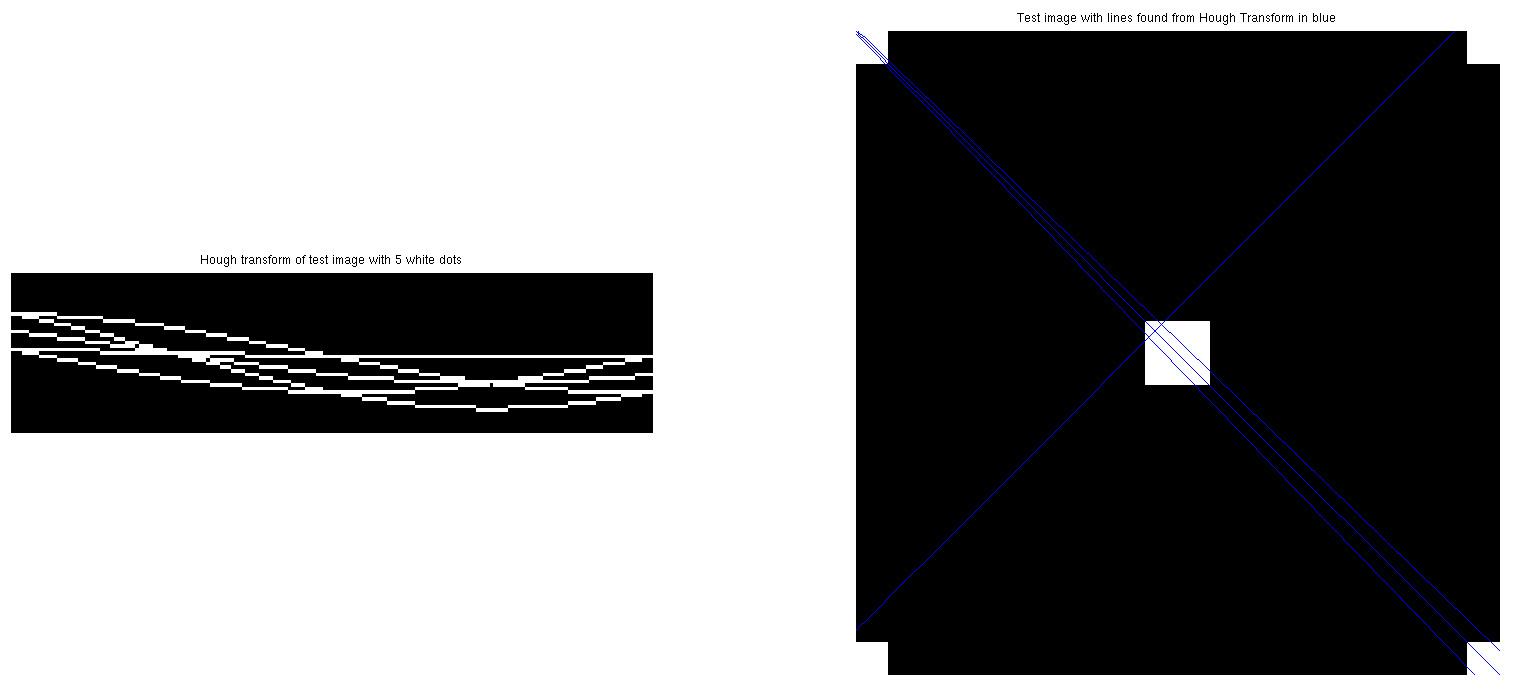
\includegraphics[width=7.5in]{1b.png}
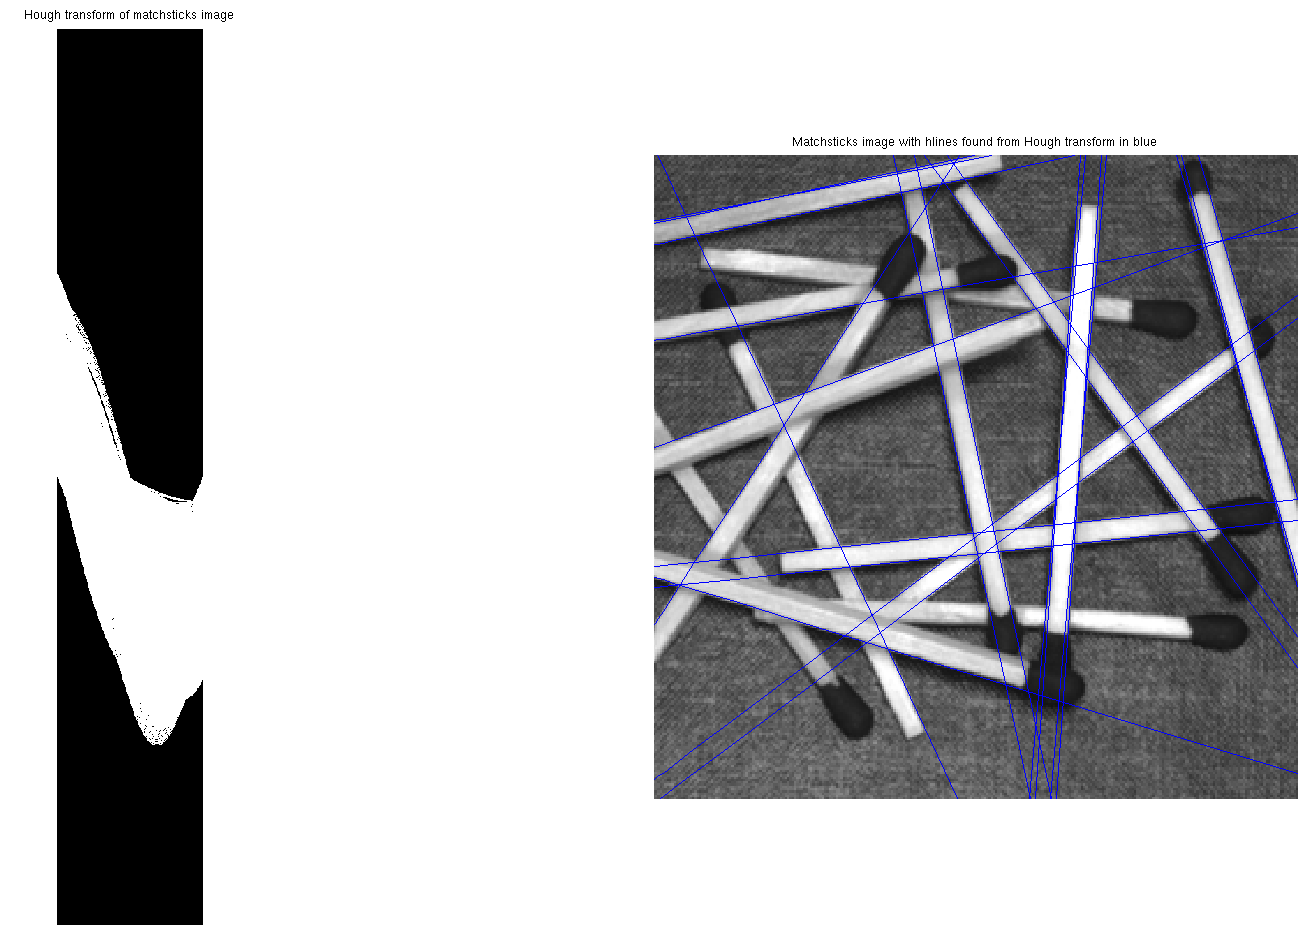
\includegraphics[width=7.5in]{1c.png}
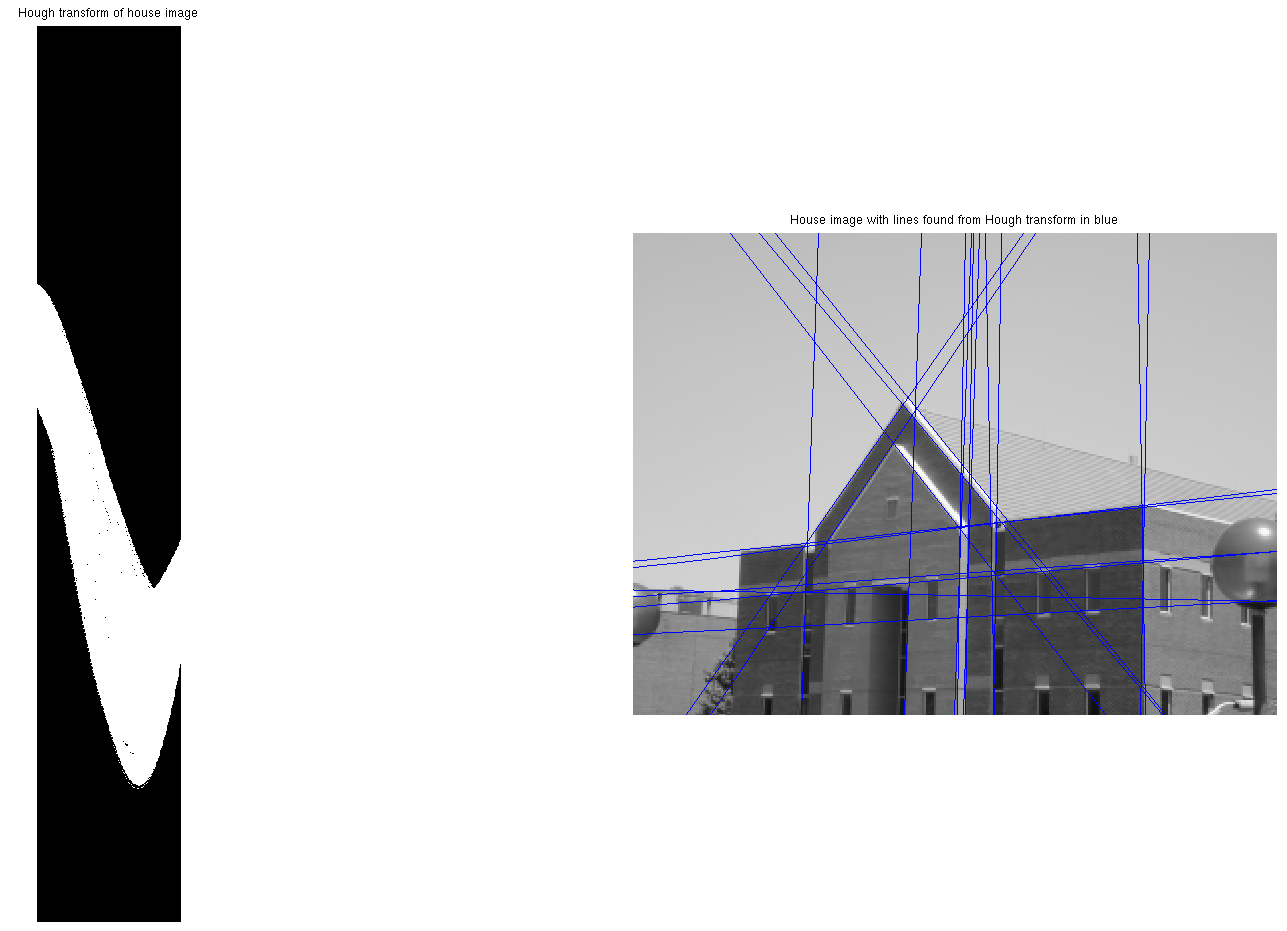
\includegraphics[width=7.5in]{1d.png}
\newpage
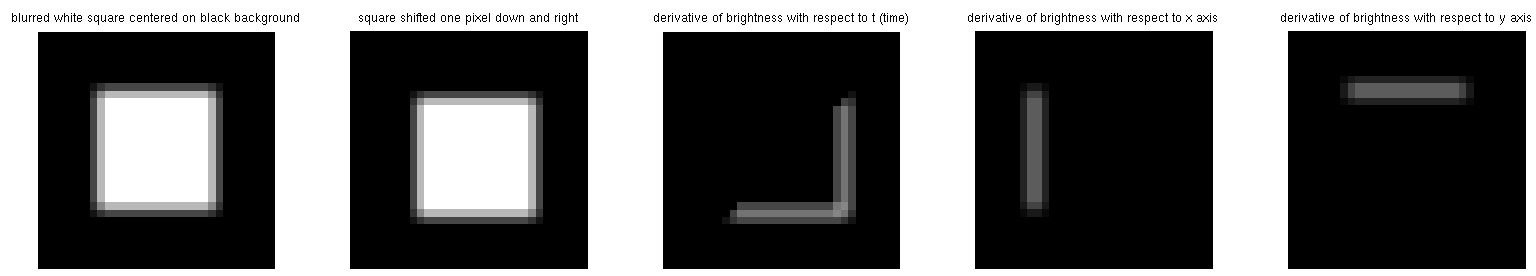
\includegraphics[width=7.5in]{2b.png}
\newline\newline\newline\newline\newline
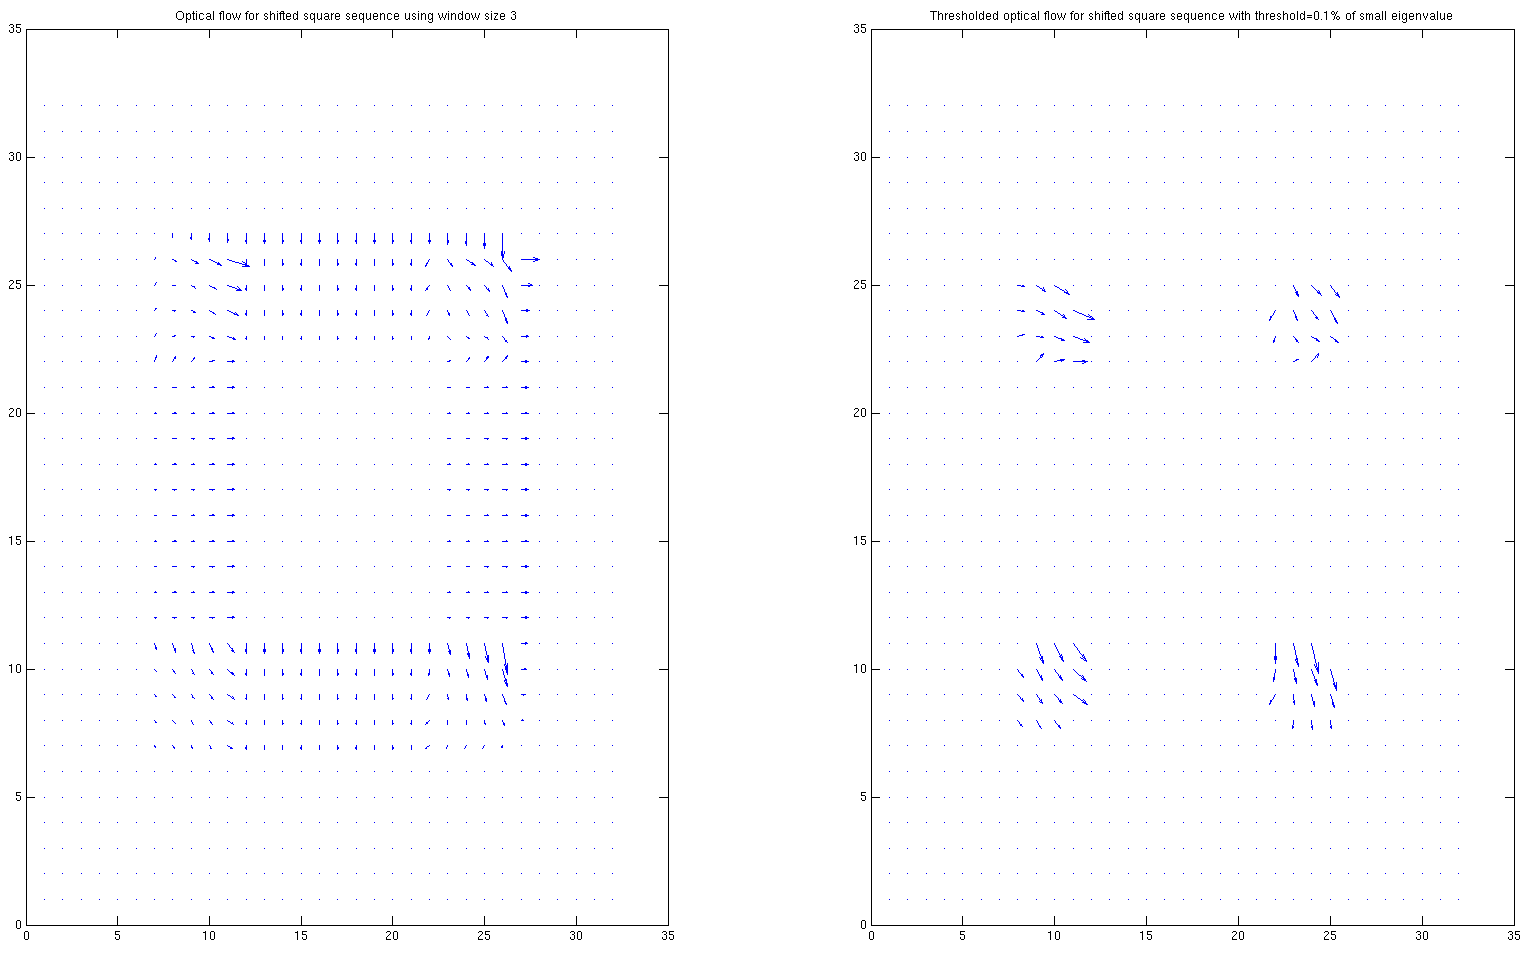
\includegraphics[width=7.5in]{2c.png}
\newpage
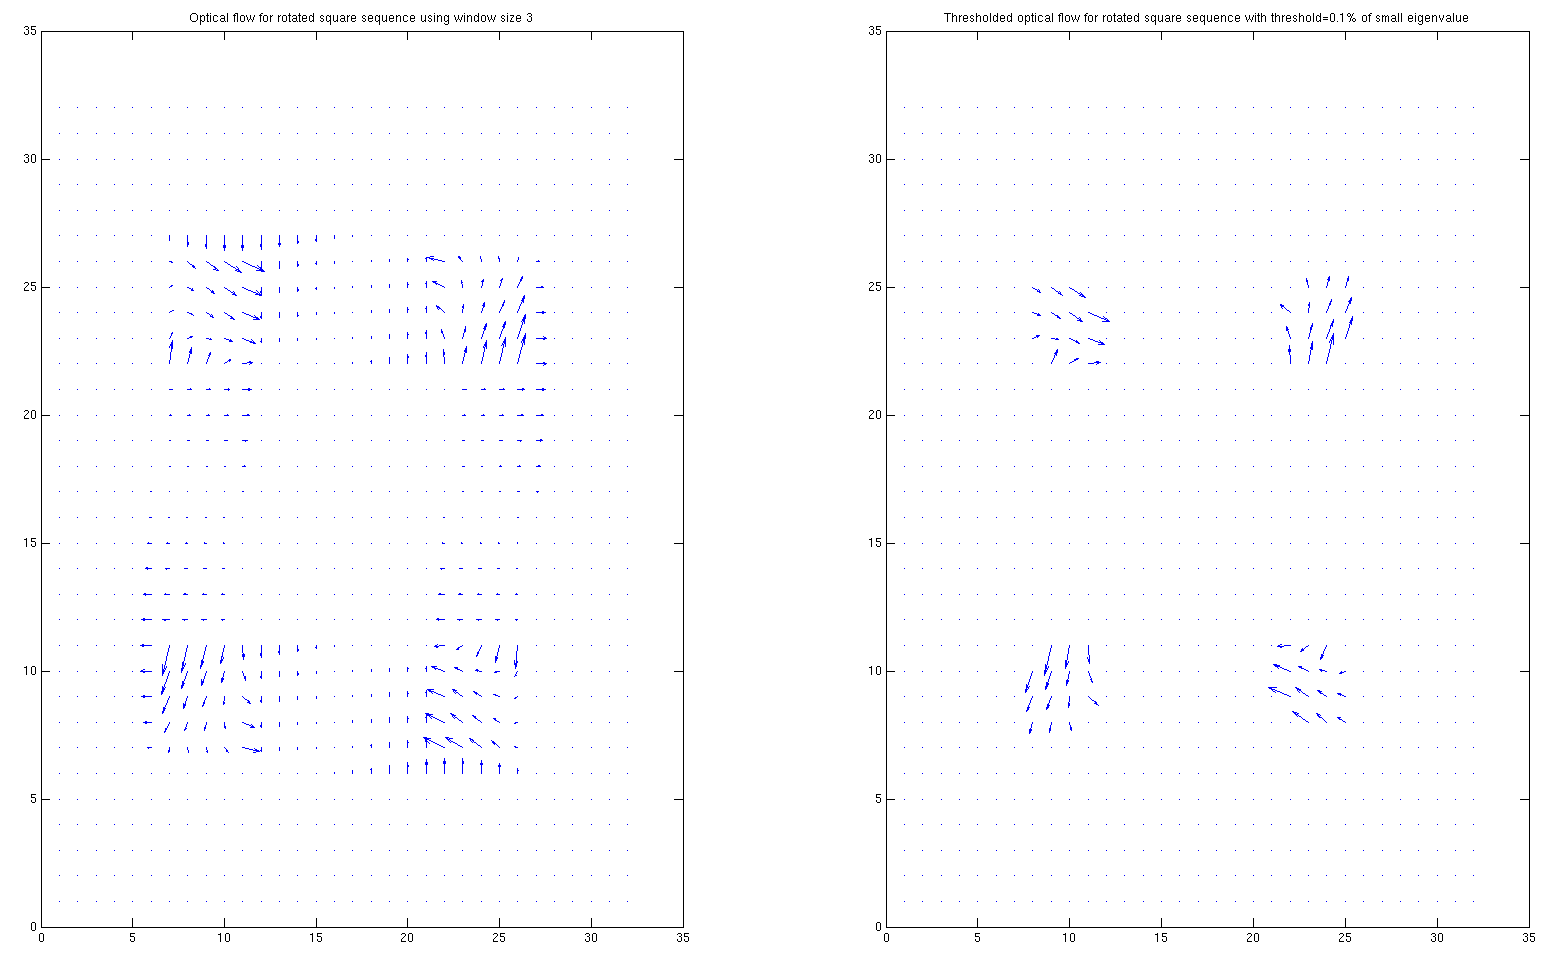
\includegraphics[width=7.5in]{2d.png}

%% CODE %%
\newpage
\begin{verbatim}
% Author: <njoffe@ucsd.edu> Nitay Joffe
% Date: 11/30/2006
% Class: CSE 166 - Image Processing
% Homework: 7
% Problem: 1 - Hough Transform
% Question: a

% (a) Implement the Hough Transform (HT) using the (\rho, \theta)
%     parameterization as described in GW Section 10.2.2. Use accumulator cells
%     with a resolution of 1 degree in \theta and 1 pixel in \rho.
function [hough_space,rho_max,theta_max] = hough_transform(binary_image)
  theta_min=-90;
  theta_max=90;
  theta=theta_min:theta_max;
  cosine_theta=cosd(theta);
  sine_theta=sind(theta);

  [ones_y,ones_x]=find(binary_image);
  ones_size=numel(ones_x);
  for i=1:numel(ones_x)
    rho(i,:)=round(ones_x(i)*cosine_theta+ones_y(i)*sine_theta);
  end
  [image_rows,image_columns]=size(binary_image);
  diagonal_distance=sqrt(image_rows^2+image_columns^2);
  rho_max=round(sqrt(2)*diagonal_distance);

  rho=rho+rho_max+1;
  theta=theta+theta_max+1;

  rho_size=rho_max*2+1;
  theta_size=numel(theta);
  hough_space=zeros(rho_size,theta_size);
  for i=1:ones_size
    for j=1:theta_size
      hough_space(rho(i,j),theta(j))=hough_space(rho(i,j),theta(j))+1;
    end
  end
end
\end{verbatim}
\newpage
\begin{verbatim}
% Author: <njoffe@ucsd.edu> Nitay Joffe
% Date: 11/30/2006
% Class: CSE 166 - Image Processing
% Homework: 7
% Problem: 1 - Hough Transform
% Questions: b,c,d
clear;

% (b) Produce a simple 11 x 11 test image made up of zeros with 5 ones in it,
%     arranged like the 5 points in GW Figure 10.20(a).
test_image=zeros(11,11);
test_image(1,1)=1;
test_image(6,6)=1;
test_image(11,1)=1;
test_image(1,11)=1;
test_image(11,11)=1;

% Compute and display its HT; the result should look like GW Figure 10.20(b).
[test_image_ht,rho_max,theta_max]=hough_transform(test_image);

% Now threshold the HT to find the (\rho, \theta)-coordinates of cells with more
% than 2 votes and plot the corresponding lines in (x, y)-space on top of the
% original image.
[rho,theta]=find(test_image_ht>2);
rho=rho-rho_max-1;
theta=theta-theta_max-1;

[test_image_y_limit test_image_x_limit]=size(test_image);
test_image_line_functions=cell(numel(rho),1);
for i=1:numel(rho)
  test_image_line_functions{i}=@(x)(rho(i)-x.*cosd(theta(i)))/sind(theta(i));
end

% (c) Load in the matchstick image in GW Figure 8.02(a) and shrink it to half
%     its size using I=imresize(I,0.5,'bil','crop');.
matchsticks_image=imread('Fig8.02(a).jpg');
matchsticks_image=imresize(matchsticks_image,0.5,'bil');

% Compute and display its edges using the Sobel operator with default threshold
% settings, i.e. BW=edge(I,'sobel');.
BW=edge(matchsticks_image,'sobel');

% Now compute and display the HT of BW. As before, threshold the HT and plot the
% corresponding lines atop the original image; this time, use a threshold of 50%
% of the maximum accumulator count over the entire HT.
[matchsticks_ht,rho_max,theta_max]=hough_transform(BW);

threshold=max(max(matchsticks_ht))/2;
[rho,theta]=find(matchsticks_ht>threshold);
rho=rho-rho_max-1;
theta=theta-theta_max-1;

[matchsticks_y_limit matchsticks_x_limit]=size(BW);
matchsticks_line_functions=cell(numel(rho),1);
for i=1:numel(rho)
  matchsticks_line_functions{i}=@(x)(rho(i)-x.*cosd(theta(i)))/sind(theta(i));
end

% (d) Repeat the previous step for another image of your choice. The image can
%     be from the textbook or elsewhere, but its size must be at least 128x128
%     and it should contain several extended straight lines.
house_image=imread('Fig10.10(a).jpg');
house_image=imresize(house_image,0.2,'bil');
BW=edge(house_image,'sobel');
[house_image_ht,rho_max,theta_max]=hough_transform(BW);

threshold=max(max(house_image_ht))/2;
[rho,theta]=find(house_image_ht>threshold);
rho=rho-rho_max-1;
theta=theta-theta_max-1;

[house_y_limit house_x_limit]=size(BW);
house_line_functions=cell(numel(rho),1);
for i=1:numel(rho)
  house_line_functions{i}=@(x)(rho(i)-x.*cosd(theta(i)))/sind(theta(i));
end


figure;
subplot(1,2,1);
imshow(test_image_ht);
title('Hough transform of test image with 5 white dots');
subplot(1,2,2);
imshow(test_image);
hold on;
for i=1:numel(test_image_line_functions)
  fplot(test_image_line_functions{i},[1 test_image_x_limit 1 test_image_y_limit]);
end
title('Test image with lines found from Hough Transform in blue');

figure;
subplot(1,2,1);
imshow(matchsticks_ht);
title('Hough transform of matchsticks image');
subplot(1,2,2);
imshow(matchsticks_image);
hold on;
for i=1:numel(matchsticks_line_functions)
  fplot(matchsticks_line_functions{i},[1 matchsticks_x_limit 1 matchsticks_y_limit]);
end
title('Matchsticks image with hlines found from Hough transform in blue');

figure;
subplot(1,2,1);
imshow(house_image_ht);
title('Hough transform of house image');
subplot(1,2,2);
imshow(house_image);
hold on;
for i=1:numel(house_line_functions)
  fplot(house_line_functions{i},[1 house_x_limit 1 house_y_limit]);
end
title('House image with lines found from Hough transform in blue');
\end{verbatim}
\newpage
\begin{verbatim}
% Author: <njoffe@ucsd.edu> Nitay Joffe
% Date: 11/30/2006
% Class: CSE 166 - Image Processing
% Homework: 7
% Problem: 2 - Lucas-Kanader optical flow
% Question: a

% Implement the Lucas-Kanade algorithm for measuring optical flow, as
% described in class. Allow the user to specify the size of the window used
% in enforcing the smoothness constraint. Use the quiver function to
% display the optical flow vectors. In addition, have your program return the
% two eigenvalues of the windowed image second moment matrix at each pixel.
function [u,v,eigenvalues_min,eigenvalues_max]=optical_flow(first_image,second_image,window_size)
  window_delta=(window_size-1)/2;
  [dx,dy]=gradient(first_image);
  dt=second_image-first_image;

  h=ones(window_size,1);
  sum_dx_squared=conv2(h,h,dx.*dx,'same');
  sum_dy_squared=conv2(h,h,dy.*dy,'same');
  sum_dx_times_dy=conv2(h,h,dx.*dy,'same');

  [rows,columns]=size(first_image);
  for i=1:rows
    for j=1:columns
      window_rows=max(1,i-window_delta):min(rows,i+window_delta);
      window_columns=max(1,j-window_delta):min(columns,j+window_delta);

      dx_window=dx(window_rows,window_columns);
      dy_window=dy(window_rows,window_columns);
      dt_window=dt(window_rows,window_columns);

      A=[dx_window(:),dy_window(:)];
      b=dt_window(:);

      scatter_matrix=[sum_dx_squared(i,j),sum_dx_times_dy(i,j);
                      sum_dx_times_dy(i,j),sum_dy_squared(i,j)];
      eigenvalues=eig(scatter_matrix);
      eigenvalues_min(i,j)=min(eigenvalues);
      eigenvalues_max(i,j)=max(eigenvalues);

      gradient_vector=-A\b;
      
      u(i,j)=gradient_vector(1);
      v(i,j)=-gradient_vector(2);      
    end
  end
end
\end{verbatim}
\newpage
\begin{verbatim}
% Author: <njoffe@ucsd.edu> Nitay Joffe
% Date: 11/30/2006
% Class: CSE 166 - Image Processing
% Homework: 7
% Problem: 2 - Lucas-Kanader optical flow
% Questions: b,c,d
clear;

% (b) Construct two frames of a simple motion sequence as follows. Make a 16x16
%     white square centered on a black background of size 32 x 32.
square_image=zeros(32);
square_image(9:24,9:24)=1;

% Blur it with a Gaussian filter with \sigma = 1.
gaussian_filter=fspecial('gaussian',3,1);
blurred_square=conv2(square_image,gaussian_filter,'same');

% This image represents I(x, y, t).
I=blurred_square;

% Produce the second image, representing I(x, y, t + 1), by displacing the first
% image down one pixel and to the right one pixel.
I_shifted=circshift(I,[1 1]);

% Display each frame, as well as I_t and the two components of \gradient(I).
[shifted_dx shifted_dy]=gradient(I);
shifted_dt=I_shifted-I;

% (c) Compute and display the optical flow for the above sequence using a window
%     size of 5 x 5.
window_size=3;
[I_shifted_u,I_shifted_v,I_shifted_eigenvalues_min]=optical_flow(I,I_shifted,window_size);

% Since you know the "ground truth" displacement (i.e. u = 1, v = 1), comment
% on the accuracy of your measured optical flow at various points throughout the
% image.

% Demonstrate how, by applying a threshold on the eigenvalues, you can suppress
% the flow vectors at pixels that suffer from the aperture problem.
threshold_percentage=0.1;
threshold=threshold_percentage*max(max(I_shifted_eigenvalues_min));

I_shifted_u_thresholded=I_shifted_u;
I_shifted_v_thresholded=I_shifted_v;

[rows,columns]=size(I_shifted_u);
for i=1:rows
  for j=1:columns
    if I_shifted_eigenvalues_min(i,j)<=threshold
      I_shifted_u_thresholded(i,j)=0;
      I_shifted_v_thresholded(i,j)=0;
    end
  end
end

% (d) Construct a new sequence consisting of the original first frame and a
%     second frame produced by rotating the first one by 5degrees (use imrotate
%     with the 'bil' and 'crop' options).
I_rotated=imrotate(I,5,'bil','crop');

% Now repeat step 2c using this sequence.
[I_rotated_u,I_rotated_v,I_rotated_eigenvalues_min]=optical_flow(I,I_rotated,window_size);

threshold=threshold_percentage*max(max(I_rotated_eigenvalues_min));

I_rotated_u_thresholded=I_rotated_u;
I_rotated_v_thresholded=I_rotated_v;

[rows,columns]=size(I_rotated_u);
for i=1:rows
  for j=1:columns
    if I_rotated_eigenvalues_min(i,j)<=threshold
      I_rotated_u_thresholded(i,j)=0;
      I_rotated_v_thresholded(i,j)=0;
    end
  end
end


figure;
subplot(1,5,1);
imshow(I);
title('blurred white square centered on black background');
subplot(1,5,2);
imshow(I_shifted);
title('square shifted one pixel down and right');
subplot(1,5,3);
imshow(shifted_dt);
title('derivative of brightness with respect to t (time)');
subplot(1,5,4);
imshow(shifted_dx);
title('derivative of brightness with respect to x axis');
subplot(1,5,5);
imshow(shifted_dy);
title('derivative of brightness with respect to y axis');

figure;
subplot(1,2,1);
quiver(I_shifted_u,I_shifted_v);
title(['Optical flow for shifted square sequence using window size ' num2str(window_size)]);
subplot(1,2,2);
quiver(I_shifted_u_thresholded,I_shifted_v_thresholded);
title(['Thresholded optical flow for shifted square sequence with threshold=' num2str(threshold_percentage) '% of small eigenvalue']);

figure;
subplot(1,2,1);
quiver(I_rotated_u,I_rotated_v);
title(['Optical flow for rotated square sequence using window size ' num2str(window_size)]);
subplot(1,2,2);
quiver(I_rotated_u_thresholded,I_rotated_v_thresholded);
title(['Thresholded optical flow for rotated square sequence with threshold=' num2str(threshold_percentage) '% of small eigenvalue']);
\end{verbatim}

\end{document}
